\tikzset{every picture/.style={line width=0.75pt}} %set default line width to 0.75pt        

\trimbox{0cm 0cm 0cm 1.8cm}{ 
	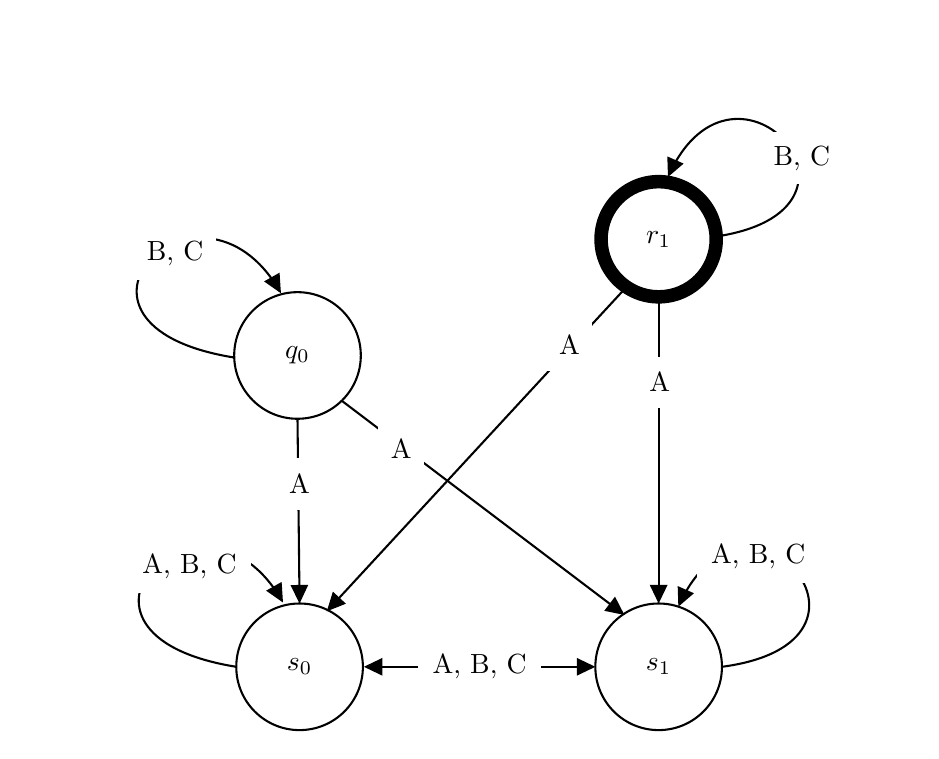
\begin{tikzpicture}[x=0.75pt,y=0.75pt,yscale=-1,xscale=1]
	%uncomment if require: \path (0,369); %set diagram left start at 0, and has height of 369
	
	%Shape: Circle [id:dp4758801382807807] 
	\draw   (93.5,322) .. controls (93.5,305.16) and (107.16,291.5) .. (124,291.5) .. controls (140.84,291.5) and (154.5,305.16) .. (154.5,322) .. controls (154.5,338.84) and (140.84,352.5) .. (124,352.5) .. controls (107.16,352.5) and (93.5,338.84) .. (93.5,322) -- cycle ;
	%Shape: Circle [id:dp5495909764900969] 
	\draw   (266.5,322) .. controls (266.5,305.16) and (280.16,291.5) .. (297,291.5) .. controls (313.84,291.5) and (327.5,305.16) .. (327.5,322) .. controls (327.5,338.84) and (313.84,352.5) .. (297,352.5) .. controls (280.16,352.5) and (266.5,338.84) .. (266.5,322) -- cycle ;
	%Straight Lines [id:da0065340714279329415] 
	\draw    (157,322) -- (264.5,322) ;
	\draw [shift={(266.5,322)}, rotate = 180] [fill={rgb, 255:red, 0; green, 0; blue, 0 }  ][line width=0.75]  [draw opacity=0] (8.93,-4.29) -- (0,0) -- (8.93,4.29) -- cycle    ;
	\draw [shift={(155,322)}, rotate = 0] [fill={rgb, 255:red, 0; green, 0; blue, 0 }  ][line width=0.75]  [draw opacity=0] (8.93,-4.29) -- (0,0) -- (8.93,4.29) -- cycle    ;
	%Curve Lines [id:da8764232980193448] 
	\draw    (93.5,322) .. controls (-5.5,306.08) and (76.67,223.33) .. (115.42,289.98) ;
	\draw [shift={(116,291)}, rotate = 240.66] [fill={rgb, 255:red, 0; green, 0; blue, 0 }  ][line width=0.75]  [draw opacity=0] (8.93,-4.29) -- (0,0) -- (8.93,4.29) -- cycle    ;
	
	%Curve Lines [id:da9911776319478228] 
	\draw    (327.5,322) .. controls (417.91,310.08) and (339.16,221.57) .. (306.98,291.93) ;
	\draw [shift={(306.5,293)}, rotate = 293.78] [fill={rgb, 255:red, 0; green, 0; blue, 0 }  ][line width=0.75]  [draw opacity=0] (8.93,-4.29) -- (0,0) -- (8.93,4.29) -- cycle    ;
	
	%Shape: Circle [id:dp7209538961655225] 
	\draw  [fill={rgb, 255:red, 0; green, 0; blue, 0 }  ,fill opacity=1 ] (266.5,116) .. controls (266.5,99.16) and (280.16,85.5) .. (297,85.5) .. controls (313.84,85.5) and (327.5,99.16) .. (327.5,116) .. controls (327.5,132.84) and (313.84,146.5) .. (297,146.5) .. controls (280.16,146.5) and (266.5,132.84) .. (266.5,116) -- cycle ;
	%Shape: Circle [id:dp27685421107424146] 
	\draw   (92.5,172) .. controls (92.5,155.16) and (106.16,141.5) .. (123,141.5) .. controls (139.84,141.5) and (153.5,155.16) .. (153.5,172) .. controls (153.5,188.84) and (139.84,202.5) .. (123,202.5) .. controls (106.16,202.5) and (92.5,188.84) .. (92.5,172) -- cycle ;
	%Shape: Circle [id:dp22158231372598314] 
	\draw  [fill={rgb, 255:red, 255; green, 255; blue, 255 }  ,fill opacity=1 ] (272,116) .. controls (272,102.19) and (283.19,91) .. (297,91) .. controls (310.81,91) and (322,102.19) .. (322,116) .. controls (322,129.81) and (310.81,141) .. (297,141) .. controls (283.19,141) and (272,129.81) .. (272,116) -- cycle ;
	%Straight Lines [id:da40013428570885556] 
	\draw    (144.3,193.8) -- (278.91,295.79) ;
	\draw [shift={(280.5,297)}, rotate = 217.15] [fill={rgb, 255:red, 0; green, 0; blue, 0 }  ][line width=0.75]  [draw opacity=0] (8.93,-4.29) -- (0,0) -- (8.93,4.29) -- cycle    ;
	
	%Straight Lines [id:da31319417430186725] 
	\draw    (281.5,139) -- (138.48,293.78) ;
	\draw [shift={(137.13,295.25)}, rotate = 312.74] [fill={rgb, 255:red, 0; green, 0; blue, 0 }  ][line width=0.75]  [draw opacity=0] (8.93,-4.29) -- (0,0) -- (8.93,4.29) -- cycle    ;
	
	%Straight Lines [id:da24005875384214737] 
	\draw    (123,202.5) -- (123.98,289.5) ;
	\draw [shift={(124,291.5)}, rotate = 269.36] [fill={rgb, 255:red, 0; green, 0; blue, 0 }  ][line width=0.75]  [draw opacity=0] (8.93,-4.29) -- (0,0) -- (8.93,4.29) -- cycle    ;
	
	%Straight Lines [id:da7741558521862318] 
	\draw    (297,146.5) -- (297,289.5) ;
	\draw [shift={(297,291.5)}, rotate = 270] [fill={rgb, 255:red, 0; green, 0; blue, 0 }  ][line width=0.75]  [draw opacity=0] (8.93,-4.29) -- (0,0) -- (8.93,4.29) -- cycle    ;
	
	%Shape: Circle [id:dp41523883310129905] 
	%\draw   (133.5,78) .. controls (133.5,61.16) and (147.16,47.5) .. (164,47.5) .. controls (180.84,47.5) and (194.5,61.16) .. (194.5,78) .. controls (194.5,94.84) and (180.84,108.5) .. (164,108.5) .. controls (147.16,108.5) and (133.5,94.84) .. (133.5,78) -- cycle ;
	%Curve Lines [id:da8202719280397651] 
	%\draw    (194.5,78) .. controls (284.91,66.08) and (206.16,-22.43) .. (173.98,47.93) ;
	%\draw [shift={(173.5,49)}, rotate = 293.78] [fill={rgb, 255:red, 0; green, 0; blue, 0 }  ][line width=0.75]  [draw opacity=0] (8.93,-4.29) -- (0,0) -- (8.93,4.29) -- cycle    ;
	
	%Curve Lines [id:da5631597181878643] 
	\draw    (322.5,115) .. controls (412.91,103.08) and (334.16,14.57) .. (301.98,84.93) ;
	\draw [shift={(301.5,86)}, rotate = 293.78] [fill={rgb, 255:red, 0; green, 0; blue, 0 }  ][line width=0.75]  [draw opacity=0] (8.93,-4.29) -- (0,0) -- (8.93,4.29) -- cycle    ;
	
	%Curve Lines [id:da7961284231370371] 
	\draw    (92.5,173) .. controls (-6.5,157.08) and (75.67,74.33) .. (114.42,140.98) ;
	\draw [shift={(115,142)}, rotate = 240.66] [fill={rgb, 255:red, 0; green, 0; blue, 0 }  ][line width=0.75]  [draw opacity=0] (8.93,-4.29) -- (0,0) -- (8.93,4.29) -- cycle    ;
	
	%Straight Lines [id:da052907042750716116] 
	%\draw    (177.5,105) -- (279.55,295.24) ;
	%\draw [shift={(280.5,297)}, rotate = 241.79] [fill={rgb, 255:red, 0; green, 0; blue, 0 }  ][line width=0.75]  [draw opacity=0] (8.93,-4.29) -- (0,0) -- (8.93,4.29) -- cycle    ;
	
	%Curve Lines [id:da9891597123428996] 
	%\draw    (95.16,339.5) .. controls (-58.51,370.39) and (40.01,-87.28) .. (140.5,56) ;
	
	%\draw [shift={(97.5,339)}, rotate = 167.09] [fill={rgb, 255:red, 0; green, 0; blue, 0 }  ][line width=0.75]  [draw opacity=0] (8.93,-4.29) -- (0,0) -- (8.93,4.29) -- cycle    ;
	
	% Text Node
	\draw  [color={rgb, 255:red, 255; green, 255; blue, 255 }  ,draw opacity=1 ][fill={rgb, 255:red, 255; green, 255; blue, 255 }  ,fill opacity=1 ]  (181.75,310) -- (239.75,310) -- (239.75,334) -- (181.75,334) -- cycle  ;
	\draw (210.75,322) node   {\agent A, \agent B, \agent C};
	% Text Node
	\draw (124,322) node   {$\defemph  s_{0}$};
	% Text Node
	\draw (297,322) node   {$\defemph  s_{1}$};
	% Text Node
	\draw  [color={rgb, 255:red, 255; green, 255; blue, 255 }  ,draw opacity=1 ][fill={rgb, 255:red, 255; green, 255; blue, 255 }  ,fill opacity=1 ]  (42,262) -- (100,262) -- (100,286) -- (42,286) -- cycle  ;
	\draw (71,274) node   {\agent A, \agent B, \agent C};
	% Text Node
	\draw  [color={rgb, 255:red, 255; green, 255; blue, 255 }  ,draw opacity=1 ][fill={rgb, 255:red, 255; green, 255; blue, 255 }  ,fill opacity=1 ]  (316,257) -- (374,257) -- (374,281) -- (316,281) -- cycle  ;
	\draw (345,269) node   {\agent A, \agent B, \agent C};
	% Text Node
	\draw (297,116) node   {$\defemph   r_{1}$};
	% Text Node
	\draw (123,172) node   {$\defemph  q_{0}$};
	% Text Node
	%\draw (164,78) node   {$\defemph  r_{1}$};
	% Text Node
	%\draw  [color={rgb, 255:red, 255; green, 255; blue, 255 }  ,draw opacity=1 ][fill={rgb, 255:red, 255; green, 255; blue, 255 }  ,fill opacity=1 ]  (213,27) -- (251,27) -- (251,51) -- (213,51) -- cycle  ;
	%\draw (232,39) node   {\agent B, \agent C};
	% Text Node
	\draw  [color={rgb, 255:red, 255; green, 255; blue, 255 }  ,draw opacity=1 ][fill={rgb, 255:red, 255; green, 255; blue, 255 }  ,fill opacity=1 ]  (243.5,155) -- (264.5,155) -- (264.5,179) -- (243.5,179) -- cycle  ;
	\draw (254,167) node   {\agent A};
	% Text Node
	\draw  [color={rgb, 255:red, 255; green, 255; blue, 255 }  ,draw opacity=1 ][fill={rgb, 255:red, 255; green, 255; blue, 255 }  ,fill opacity=1 ]  (287,173) -- (308,173) -- (308,197) -- (287,197) -- cycle  ;
	\draw (297.5,185) node   {\agent A};
	% Text Node
	%\draw  [color={rgb, 255:red, 255; green, 255; blue, 255 }  ,draw opacity=1 ][fill={rgb, 255:red, 255; green, 255; blue, 255 }  ,fill opacity=1 ]  (194.5,139) -- (215.5,139) -- (215.5,163) -- (194.5,163) -- cycle  ;
	%\draw (205,151) node   {\agent A};
	% Text Node
	\draw  [color={rgb, 255:red, 255; green, 255; blue, 255 }  ,draw opacity=1 ][fill={rgb, 255:red, 255; green, 255; blue, 255 }  ,fill opacity=1 ]  (113.5,222) -- (134.5,222) -- (134.5,246) -- (113.5,246) -- cycle  ;
	\draw (124,234) node   {\agent A};
	% Text Node
	\draw  [color={rgb, 255:red, 255; green, 255; blue, 255 }  ,draw opacity=1 ][fill={rgb, 255:red, 255; green, 255; blue, 255 }  ,fill opacity=1 ]  (162.5,205) -- (183.5,205) -- (183.5,229) -- (162.5,229) -- cycle  ;
	\draw (173,217) node   {\agent A};
	% Text Node
	\draw  [color={rgb, 255:red, 255; green, 255; blue, 255 }  ,draw opacity=1 ][fill={rgb, 255:red, 255; green, 255; blue, 255 }  ,fill opacity=1 ]  (347,65) -- (385,65) -- (385,89) -- (347,89) -- cycle  ;
	\draw (366,77) node   {\agent B, \agent C};
	% Text Node
	\draw  [color={rgb, 255:red, 255; green, 255; blue, 255 }  ,draw opacity=1 ][fill={rgb, 255:red, 255; green, 255; blue, 255 }  ,fill opacity=1 ]  (45,111) -- (83,111) -- (83,135) -- (45,135) -- cycle  ;
	\draw (64,123) node   {\agent B, \agent C};
	% Text Node
	%\draw  [color={rgb, 255:red, 255; green, 255; blue, 255 }  ,draw opacity=1 ][fill={rgb, 255:red, 255; green, 255; blue, 255 }  ,fill opacity=1 ]  (46.5,48) -- (67.5,48) -- (67.5,72) -- (46.5,72) -- cycle  ;
	%\draw (57,60) node   {\agent A};
	
	
	\end{tikzpicture}
}